\section{Solver, penalty and recovery details}
\label{app:details}
This appendix keeps the detailed solver-side results that the main text summarises in \cref{sec:penaltysummary}.

\subsection{Functional checks of the recovery and penalty integration}
\label{sec:integrationchecks}
The initial integration passed 98 local automated tests, including 14 tests for the penalty integration.
The expanded suite now passes 111 tests, adding data contracts, requirement coverage and workflow recovery checks.
These checks establish behaviour on fixtures, not application-level performance. The compiler tests enumerate
small binary, unary-slack and unbalanced encodings and compare PyQUBO energies with the native compiler at
multiple weights. They also check constant-only models, unused variables, compilation reuse, and the distinction
between original feasibility and encoded slack diagnostics.

For all four penalty-only policies, a stopped-and-resumed local SA run reproduces the configuration sequence
and best solution of an uninterrupted run, with completed calls retained in the cumulative budget. Additional
checks reject changed-model and unresolved-call checkpoints, bound grid enumeration and retain feasible-result
stopping on resume. Recovery fixtures cover invalid or infeasible models, bounded repairs, baseline delivery,
artifact rollback and generated-code timeouts. Acquisition tests use controlled download failures; they do not
exercise live web services or live LLM routing.

A separate command-line SA check continued a two-round cross-entropy search for two further rounds, reporting
four cumulative calls. UI checks produced a saved result for a feasible fixture and a failure report with zero
annealer calls for an infeasible fixture. A UI resume check retained one completed call and continued to
three cumulative calls. At that stage no additional real-hardware experiment had been performed for this integration;
subsequent actual-backend experiments are reported in \cref{sec:additionalexperiments}.
The performance results in \cref{sec:tuningcomparison} precede these new policies.

A separate pilot compares default and rule policies with the four new penalty policies on eight synthetic
knapsack and select-k instances, with three seeds per instance. All 144 local SA runs completed without
crashes under a six-call ceiling (60 reads and 300 sweeps per call). Mean gaps were 0.0853 for default,
0.1135 for rule, and 0.1107, 0.1063, 0.1413 and 0.0980 for TPE, grid, cross-entropy and sequential search,
respectively. Early stopping gave different actual call counts. None of the new policies improved on
default mean gap in this small comparison; it does not establish superiority on applications or hardware.

In a controlled recovery experiment, four injected repairable faults were each tested on three coefficient
seeds. Without a correction callback, none of the 12 cases delivered a solution; with a callback restoring
the known fixture, all 12 delivered one. Both conditions rejected all three attempts to change a fixed user
setting. These results check recovery control and validation, not LLM diagnosis quality.

A real-data pilot downloaded the official UCI Wine Quality archive\footnote{\url{https://archive.ics.uci.edu/dataset/186/wine+quality}} and used all 1,599 red-wine records.
The local model generated both model and adapter code. An independent audit recomputed correlations and
checked objective and cardinality against all 2,048 binary assignments. The pilot selected five
features with objective 0.7497088247, matching the enumerated optimum after four SA calls. Failed attempts
are retained: model generation sometimes named a nonexistent mapped constraint, source ranking rejected
the official archive, and the adapter omitted metadata or marked descriptions as assumptions. The successful
recovery run reused a previously generated model and prepared-data cache, with case-specific review of
descriptive notes. After improving the validation feedback, a fresh run completed without these caches or
review items in about 64 seconds, using 20,596 LLM tokens. These runs concern one specified-source local SA
acceptance case, not a ten-case success rate or a demonstration
of unrestricted autonomous acquisition.

\subsection{Additional backend, penalty and encoding experiments}
\label{sec:additionalexperiments}
We froze the models before comparing policies and distinguish these experiments from live model generation.
The comparison uses a common solver-call ceiling within each backend; actual calls can differ through early stopping.
Compute seconds across simulated annealing and a GPU service are not equivalent resources.
\paragraph{Extended penalty comparison.}
The eight synthetic test instances were repeated with ten solver seeds under eight policies, giving 640 runs.
Each run allowed at most six calls, with 60 SA reads and 300 sweeps per call. Every run returned a feasible result.
Table~\ref{tab:extendedpenalty} reports mean gaps and hierarchical bootstrap intervals (10,000 draws, resampling
instances and then seeds within instances). Paired Wilcoxon tests use the eight per-instance seed-averaged
differences, rather than treating 80 runs as independent problems. Holm correction is applied to the four
penalty-versus-default tests. All four penalty policies had higher mean gaps than default (adjusted
$p=0.03125$). The result concerns this small fixed test set and does not establish a ranking across applications.
\begin{table}[t]\centering\small
\caption{Extended local SA comparison. Intervals are 95\% hierarchical bootstrap intervals; all policies have 80 runs.}
\label{tab:extendedpenalty}
\begin{tabular}{@{}lrrr@{}}\toprule Policy & Mean gap & 95\% interval & Calls \\\midrule
default & 0.0932 & [0.0262, 0.1598] & 4.81 \\
rule & 0.1151 & [0.0386, 0.1913] & 2.15 \\
random & 0.1396 & [0.0807, 0.1987] & 5.95 \\
optuna & 0.1322 & [0.0656, 0.1994] & 5.91 \\
penalty\_tpe & 0.1080 & [0.0409, 0.1748] & 5.88 \\
penalty\_grid & 0.1070 & [0.0309, 0.1828] & 3.44 \\
penalty\_cem & 0.1372 & [0.0881, 0.1878] & 5.94 \\
penalty\_sequential & 0.1003 & [0.0356, 0.1652] & 5.28 \\
\bottomrule\end{tabular}\end{table}
\begin{figure}[t]\centering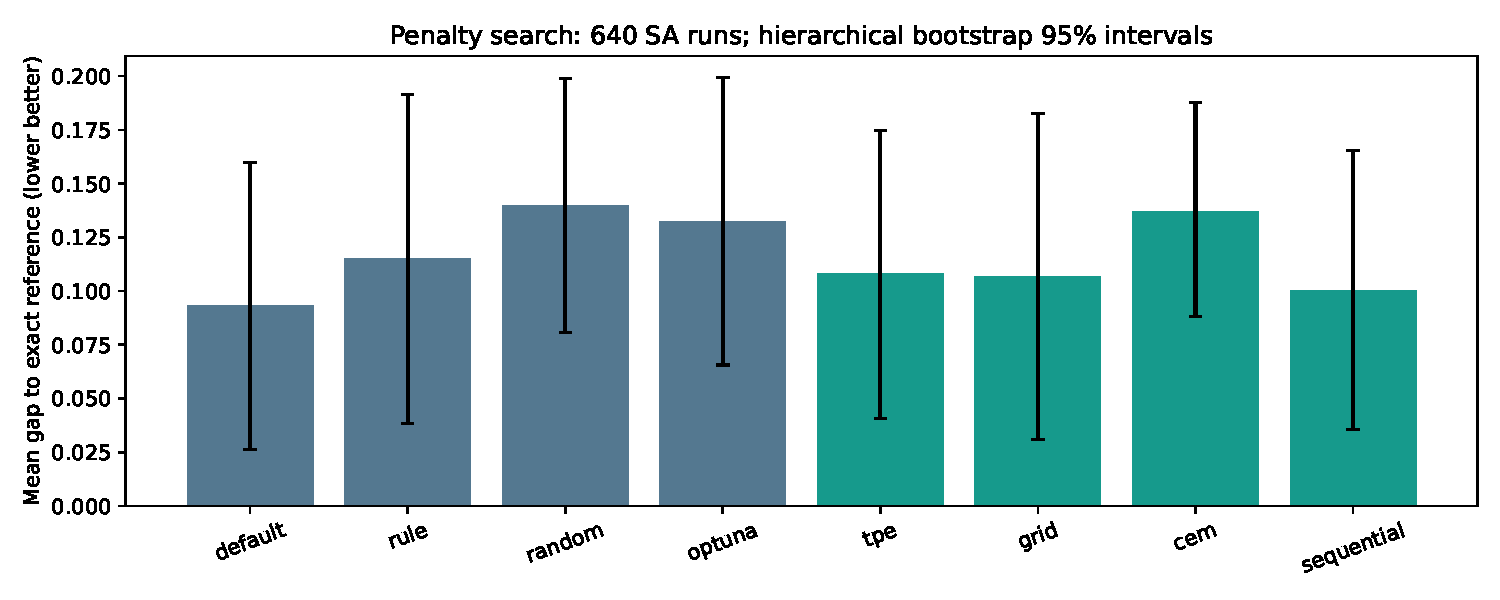
\includegraphics[width=\linewidth]{figures/penalty_comparison.pdf}
\caption{Penalty comparison on eight synthetic instances and ten seeds, separate from the earlier agent comparison.}\end{figure}
\paragraph{Actual backend calls.}
We evaluated the frozen red-wine model and generated knapsack (60 items) and conflict selection (80 items)
models under default, penalty TPE and single-agent policies, with three repetitions per condition on SA and
CGA. All 54 conditions produced feasible solutions without external-call errors. Each condition allowed
at most three calls; CGA calls used a three-second search limit, while SA used 60 reads and 300 sweeps.
External repetitions are repeated submissions, since the GPU service exposes no RNG seed.
On CGA, the red-wine mean gaps were 0.5495 for default, 0.0740 for TPE and 0.0000 for the agent.
On the other two CGA models, defaults already attained the exact reference. Agent mean end-to-end times
on CGA were 73.9--97.0 seconds per condition, versus 19.5--23.7 seconds for defaults, including network
and local inference overhead. Quality gains therefore do not imply lower wall time. Three repetitions
are insufficient to establish a general hardware advantage.
\begin{figure}[t]\centering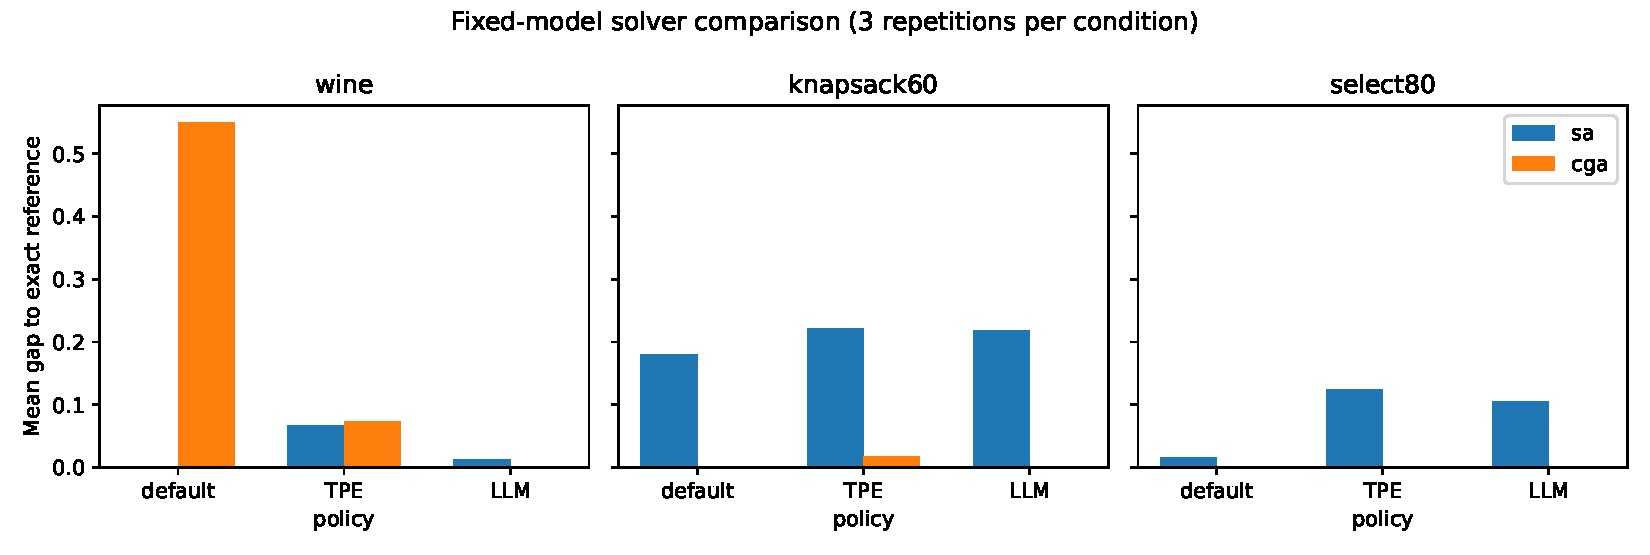
\includegraphics[width=\linewidth]{figures/backend_comparison.pdf}
\caption{Fixed-model SA and real CGA comparison, three repetitions per condition. The references are exact for these three models.}\end{figure}
An actual Fujitsu DA submission was rejected with HTTP 400 and the service message
``Monthly usage exceeds specified metering limit.'' Further submissions were withheld. This is an
external account limitation, not evidence of model infeasibility; no simulated stand-in is counted as a DA result.
\paragraph{Encoding ablation.}
Two fixed knapsack instances (12 and 30 items) were compiled with binary slack, unary slack and unbalanced
encoding, keeping original objectives, constraints, default weights and call ceilings fixed. There were
60 SA conditions (ten seeds each) and 18 actual CGA conditions (three submissions each). For 30 items,
binary, unary and unbalanced encodings used 38, 163 and 30 variables, respectively; SA mean gaps were
0.1661, 0.3250 and 0.1188. CGA attained the reference in all three encodings for that instance, but
unbalanced encoding missed the optimum on the 12-item instance (gap 0.0387). Fewer variables can help
search, but an approximate encoding does not guarantee preservation of the original optimum. These
are two instance-specific ablations, not a broad evaluation of automatic encoding selection.
\begin{figure}[t]\centering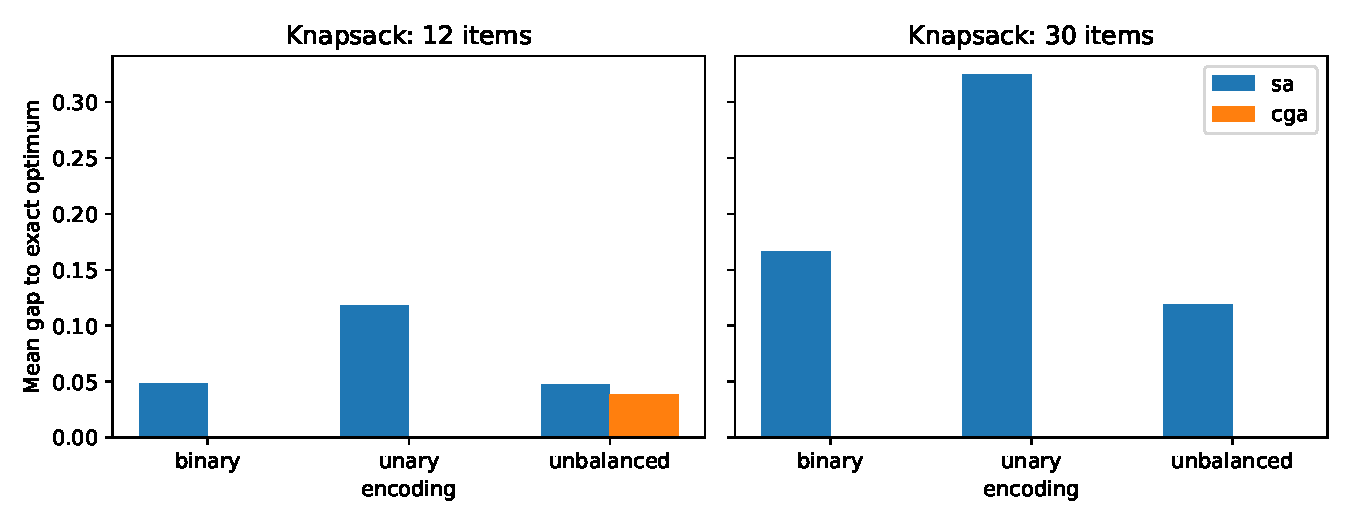
\includegraphics[width=\linewidth]{figures/encoding_comparison.pdf}
\caption{Encoding ablation with original-problem feasibility evaluation and exact knapsack references.}\end{figure}
\paragraph{A larger real-coordinate routing model.}
A fixed Taipei YouBike snapshot supplied 40 active station coordinates. A hand-written position-encoding
TSP model has 1,600 binary decision variables and was checked against direct tour evaluation on 12
valid tours. This experiment measures solving and tuning, not autonomous LLM formulation. Distances
are haversine kilometres, not road travel distances. A 20-restart 2-opt heuristic gave a feasible
7.695977-km tour; it is not a certified optimum. Each policy/backend condition was
repeated three times with a three-call ceiling (30 reads and 300 sweeps for SA, three-second CGA calls).
\begin{table}[t]\centering\small
\caption{40-station routing. Mean distances and relative differences use feasible runs only; feasibility counts report all runs. The comparison is to a feasible heuristic, not an exact optimum.}
\label{tab:largerouting}
\begin{tabular}{@{}llrrr@{}}\toprule Backend & Policy & Feasible & Mean km & Heur. gap \\\midrule
sa & default & 3/3 & 29.32 & 2.809 \\
sa & penalty\_tpe & 2/3 & 35.41 & 3.601 \\
sa & agent & 3/3 & 30.72 & 2.991 \\
cga & default & 3/3 & 25.44 & 2.306 \\
cga & penalty\_tpe & 3/3 & 26.91 & 2.496 \\
cga & agent & 3/3 & 26.03 & 2.382 \\
\bottomrule\end{tabular}\end{table}
\begin{figure}[t]\centering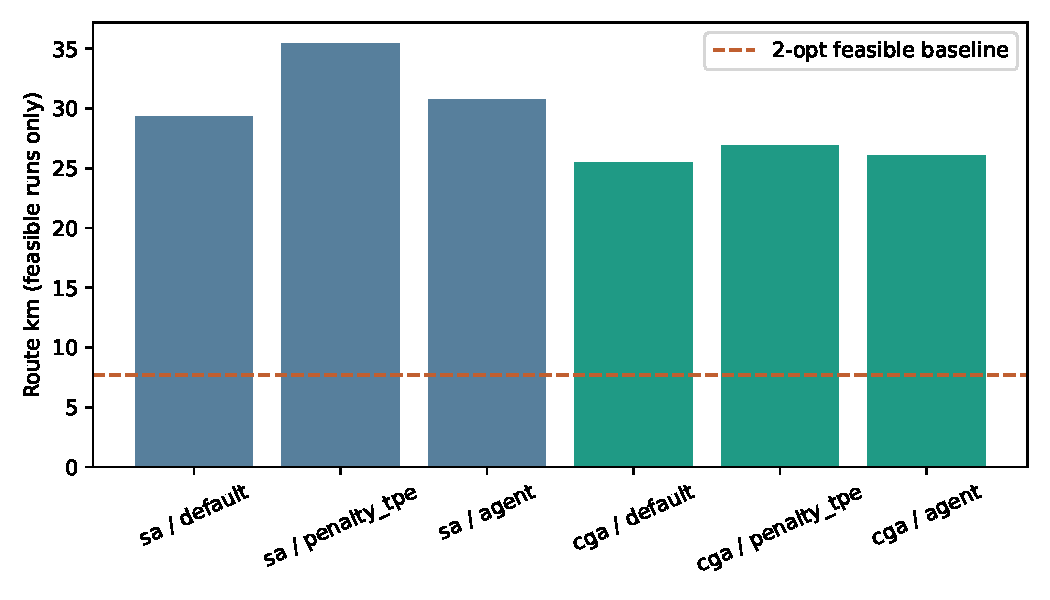
\includegraphics[width=\linewidth]{figures/routing_comparison.pdf}
\caption{Large routing quality. Missing feasible outputs are recorded separately rather than assigned an arbitrary gap.}\end{figure}
\paragraph{Additional live-data acceptance and checker corrections.}
Three fresh wine model/adapter generations were retained. The initial acceptance checker incorrectly
rejected equivalent minimization of the negative objective, required an unnecessary input field
even when the confirmed setting was embedded in the model, and loaded unrelated unreadable candidate
files. After correcting the checker, all three saved outputs passed the full 2,048-assignment audit
and delivered feasible solutions. The re-audit reused artifacts; it is not a prospective 100\% success
rate for a fixed autonomous acceptance protocol. Initial errors and corrected evaluations are both retained.
The Wholesale Customers case used the public UCI data\footnote{\url{https://archive.ics.uci.edu/dataset/292/wholesale+customers}}, a fixed sample of 24 rows and six spending
features. Independent checks reproduced the sample, log transform, standardization and distance matrix.
The recovered run formed three groups of eight, with objective 856.8319 versus a feasible baseline
of 1021.7818 (16.1\% lower). The run reused its generated model and obtained data and adapter code anew.
Failures exposed fixed-size requirement maps and an unsupported generated import of the preprocessing
module; the implementation now supports specific family-prefix mappings and tracked imports.
A recovered Zachary karate-club case used the university-published 34-node, 78-edge GML archive\footnote{\url{https://websites.umich.edu/~mejn/netdata/}}.
An independent source check rejected an adapter that sorted adjacency columns lexicographically,
permuting columns without rows. Numeric ordering restored the source matrix. The delivered split
has 17 nodes per group and 17 cut edges, using the feasible conventional baseline because annealing
returned a worse best result (22 cut edges). This is attributed baseline delivery, not an annealer
improvement. Declared descriptive notes were discharged by the case-specific independent source audit.
Recovered examples do not establish general LLM diagnosis or repair success rates.
The earlier integration snapshot passed 120 automated tests, and UI checks retained feasible/failure delivery
and cumulative checkpoint resume. After the structured-schema and checker additions, the current offline
suite passed 146 tests. Neither count establishes autonomous real-data success. Raw instances, configurations, source hashes, transcripts, error records
and standalone figure artifacts accompany the report. General requirement-semantic correctness,
a held-out backend-transfer experiment and execution of the entire ten-case catalog remain open.

\subsection{D-Wave Hybrid BQM with an explicit ten-second limit}
\label{sec:dwavehybrid}
We submitted the same three frozen models to the real Leap Hybrid BQM service, under default,
penalty TPE and single-agent policies. This service is distinct from direct QPU sampling.
The experiment completed 27 of 27 conditions and used 72 solver submissions.
Each condition allowed at most three calls. Every call explicitly set the service time limit
to ten seconds; a model requiring a larger minimum was refused before submission rather than
given a longer limit. Sequential execution was bounded by 81 calls and 810 service seconds.
A read-only retrieval of 72 completed answers reported total service charge time
of 719.495 seconds. The original ledger conservatively reserved ten seconds per call;
the answers also report 42.526 seconds of aggregate internal QPU access,
positive for 72 of 72 answers. These are hybrid-service timings, not direct-QPU runs.
measured service timings are preserved separately. Network and inference time are additional.
\begin{table}[t]\centering\small
\caption{Real Hybrid BQM comparison. Gaps use exact references for the three frozen models; wall time includes network and inference.}
\begin{tabular}{@{}llrrrr@{}}\toprule Model & Policy & Feasible & Gap & Calls & Wall s \\\midrule
wine & default & 3/3 & 0.0000 & 3.00 & 43.4 \\
wine & penalty\_tpe & 3/3 & 0.0000 & 3.00 & 43.6 \\
wine & agent & 3/3 & 0.0000 & 1.00 & 52.3 \\
knapsack60 & default & 3/3 & 0.1060 & 3.00 & 42.0 \\
knapsack60 & penalty\_tpe & 3/3 & 0.1164 & 3.00 & 41.9 \\
knapsack60 & agent & 3/3 & 0.1149 & 3.00 & 123.5 \\
select80 & default & 3/3 & 0.0000 & 3.00 & 44.8 \\
select80 & penalty\_tpe & 3/3 & 0.0141 & 3.00 & 43.6 \\
select80 & agent & 3/3 & 0.0016 & 2.00 & 97.2 \\
\bottomrule\end{tabular}\end{table}
\begin{figure}[t]\centering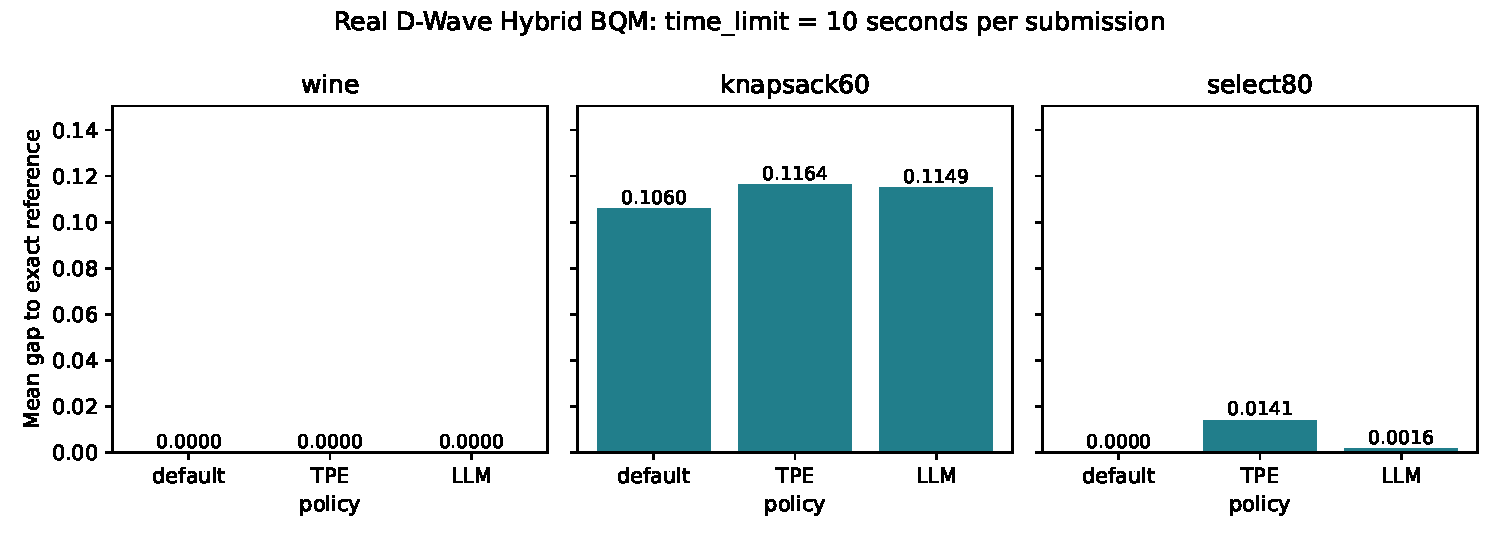
\includegraphics[width=\linewidth]{figures/dwave_hybrid_comparison.pdf}
\caption{Real hybrid-service results with an explicit ten-second limit.}\end{figure}
The three repetitions are external resubmissions, without exposed hardware RNG seeds.
The ten-second Hybrid ceiling and earlier three-second CGA ceiling are different resource
allocations. They do not establish a hardware advantage, nor a held-out knowledge-transfer result.

